\documentclass{beamer}

\usepackage{braket}
\usepackage{amsmath}
\usepackage{amssymb}
\usepackage{graphicx}
\usepackage{subcaption}
\graphicspath{ {./img/} }

\usetheme{Copenhagen}
\useoutertheme{infolines}
\usecolortheme{dolphin}

\newcommand{\comp}{\boxplus}
\newcommand{\diag}{\boxtimes}
\newcommand{\calH}{\mathcal{H}}
\newcommand{\kp}{\ket{\psi}}
\newcommand{\kf}{\ket{\phi}}
\newcommand{\kz}{\ket{0}}
\newcommand{\ko}{\ket{1}}
\newcommand{\kpl}{\ket{+}}
\newcommand{\km}{\ket{-}}
\newcommand{\oost}{\frac{1}{\sqrt{2}}}

%Information to be included in the title page:
\title{Comparing Quantum Protocols via PRISM}
\author{Gabriele Tedeschi}
\institute{University of Pisa}
\date{\today}	

\begin{document}



\frame{\titlepage}

\begin{frame}{Motivations}
Quantum cryptographic protocols have been proved to be \textbf{unconditionally secure}, meaning that every possible attack will fail with probability arbitrarily close to one.

\bigskip
But one would also like to:\begin{itemize}
\item Compare different protocols
\item Verify other properties of the protocol
\item Compare the behaviour with different parameters
\end{itemize}

\bigskip
Thats when \textbf{model checking} comes in handy!
\end{frame}

\begin{frame}
	\frametitle{Table of Contents}
	\tableofcontents
	\end{frame}


\section{Quantum computing fundamentals}
\begin{frame}%notation
\frametitle{Braket Notation}
\begin{columns}
\column{0.5\textwidth}
In linear algebra, we write:
\begin{itemize}
\item Vector $\mathbf{v}$
\item Conjugate transpose $\mathbf{v}^* = \mathbf{v}^H = \overline{\mathbf{v}^T}$
\item Dot product between $\mathbf{v}$ and $\mathbf{u}$ 
\hspace*{1.5cm}$v^* \cdot u$
\item Norm of $\mathbf{v}$: $\|\mathbf{v}\| = v^* \cdot u$

\end{itemize}
\pause
\column{0.5\textwidth}
In quantum mechanics, we write:
\begin{itemize}
\item Vector $\ket{\psi}$
\item conjugate transpose $\bra{\psi} = \ket{\psi}^H = \overline{\ket{\psi}^T}$
\item dot product between{\small  $\ket{\psi}$} and {\small $\ket{\phi}$}
\hspace*{1.5cm}$\braket{\psi | \phi}$
\item Norm of $\kp$: $\braket{\psi | \psi}$
\end{itemize}
\end{columns}
\end{frame}
\subsection{Quantum State}	
\begin{frame}%first postulate
	\frametitle{First Postulate: Quantum State}
\begin{block}{I Postulate}
	
Any \textbf{isolated} physical system	is completely described by a \textbf{unit vector} in a \textbf{complex vector space} with inner product (called \textbf{Hilbert Space} $\calH$)	
	\end{block}
		\begin{itemize}
		\pause
		\item \textbf{Complex vector space}: A vector space with coefficients in $\mathbb{C}$, so some possible vectors are: 
		\[
		\begin{pmatrix}
		1\\
		0
		\end{pmatrix},\quad
		\begin{pmatrix}
		i\\
		i
		\end{pmatrix},\quad
		\begin{pmatrix}
		5+5i\\
		\frac{1}{3} + \frac{1}{5}i
		\end{pmatrix},\quad\ldots
		\]
		\pause
		\item \textbf{Unit vector}: a vector $\kp$ such that $\braket{\psi | \psi}$ = 1, like: 
		\[
		\begin{pmatrix}
		1\\
		0
		\end{pmatrix},\quad
		\begin{pmatrix}
		0\\
		i
		\end{pmatrix},\quad
		\begin{pmatrix}
		\frac{1}{\sqrt{2}}\\
		\oost i
		\end{pmatrix},\quad\ldots
		\]
		\end{itemize}
	\end{frame}
\begin{frame}%qubits
	\frametitle{Qubits}
	Suppose a physical system with only two states: an particle with spin up or spin down, for example, or an electron that can be in an excited state or in the ground state.
\begin{figure}
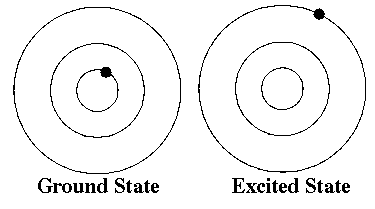
\includegraphics[scale=0.7]{states}	
\end{figure}	
	\begin{block}{Qubits}
	A system with only two possible state is described by a \textbf{qubit}, a unitary vector in the 2-dimensional Hilbert space 
	$\calH_2 \equiv \mathbb{C}^2$	.
	\end{block}
\end{frame}

\begin{frame}%qubits CONT
For example, if an electron is in the ground state, we say that is in state 
$$\ket{0} = \begin{pmatrix}
1 \\
0
\end{pmatrix}	$$

while if it is in the excited state, it's in state 
$$\ket{1} = \begin{pmatrix}
0\\
1
\end{pmatrix}$$


\begin{block}{Computational Basis}
$\ket{0}$ and $\ket{1}$ form the so called \textbf{computational base} of the (bidimensional) Hilbert space. This means that each vector $\kp$ can be expressed as
\[
	\kp = \begin{pmatrix}
	\alpha \\
	\beta
	\end{pmatrix} = \alpha\kz + \beta\ko\text{, with }\alpha, \beta \in \mathbb{C}, \braket{\psi | \psi} = 1
\]
\end{block}
\end{frame}

\begin{frame}%superposition
\frametitle{Quantum Superposition}

Since $\kz$ and $\ko$ are vectors in $\calH_2$, so it is any \textbf{linear combination} of the two, provided it has unitary length.
\[
	\begin{pmatrix}
	\oost \\
	\oost 
	\end{pmatrix}, \quad
	\begin{pmatrix}
	\oost \\
	-\oost 
	\end{pmatrix}, \quad
	\begin{pmatrix}
	\sqrt{0.9}\\
	\sqrt{0.1}
	\end{pmatrix}
\]
\pause
\begin{block}{Hadamard basis}
The vector $\begin{pmatrix}
	\oost \\
	\oost 
	\end{pmatrix} = 
	\oost\begin{pmatrix}
	1 \\
	1 
	\end{pmatrix} = 
	\oost\kz + \oost\ko$ is called the $\ket{+}$ state

The vector $\begin{pmatrix}
	\oost \\
	-\oost 
	\end{pmatrix} = 
	\oost\begin{pmatrix}
	1 \\
	.1 
	\end{pmatrix} = 
	\oost\kz - \oost\ko$ is called the $\ket{-}$ state	
	They form the Hadamard Basis of $\mathcal{H}_2$
\end{block}
\end{frame}

\begin{frame}%bloch sphere
\frametitle{Bloch sphere}
\begin{figure}
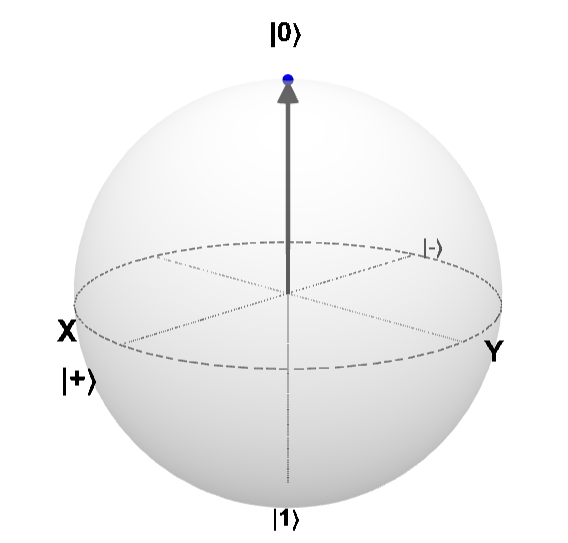
\includegraphics[scale=0.2]{ket0}\quad
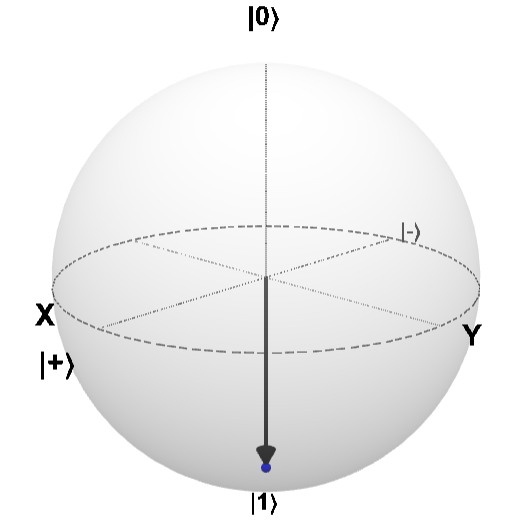
\includegraphics[scale=0.2]{ket1}
\end{figure}
\pause
\begin{figure}
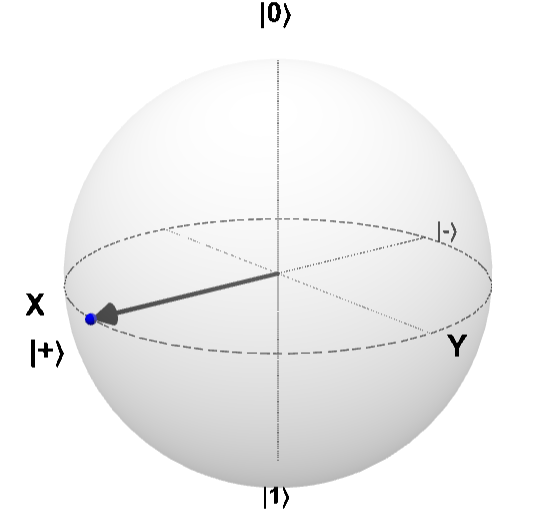
\includegraphics[scale=0.35]{ket+}\pause\quad
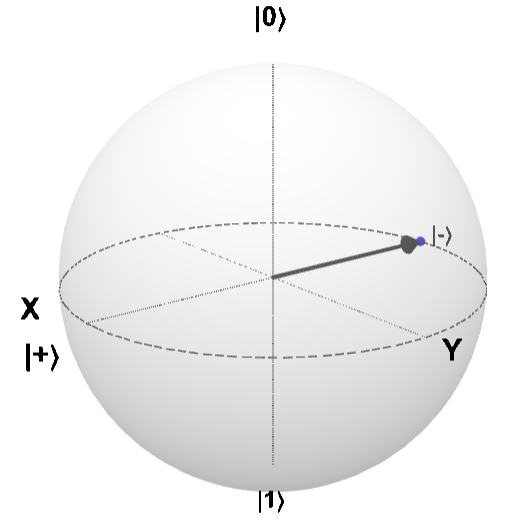
\includegraphics[scale=0.35]{ket-}
\end{figure}
\end{frame}

\begin{frame}%phase
\frametitle{Phase}
\begin{figure}
\begin{subfigure}{0.49\textwidth}
\centering
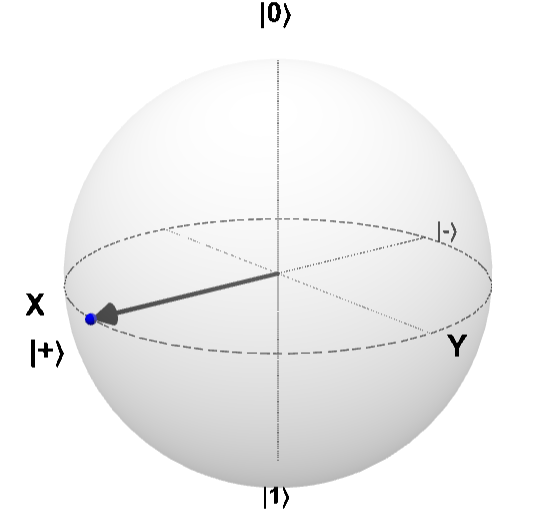
\includegraphics[scale=0.25]{ket+}
\caption*{$\ket{+} = \kz + e^{i0}\ko$}
\end{subfigure}
\begin{subfigure}{0.49\textwidth}
\centering
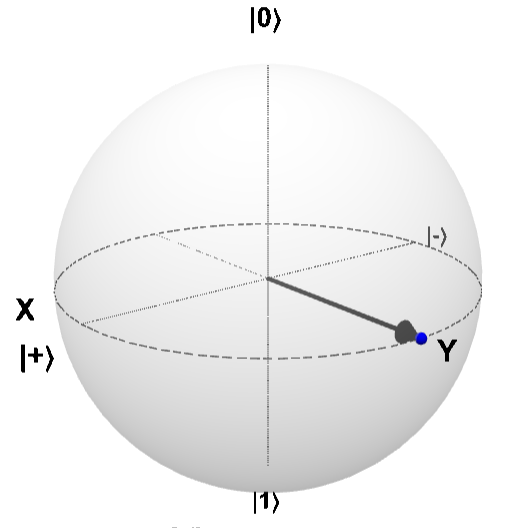
\includegraphics[scale=0.15]{zero+ione}
\caption*{$\kz + e^{i\frac{\pi}{2}}\ko$}
\end{subfigure}
\end{figure}


\begin{figure}
\begin{subfigure}{0.49\textwidth}
\centering
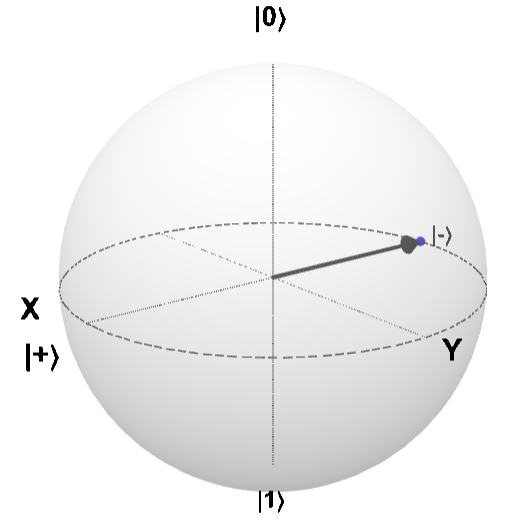
\includegraphics[scale=0.25]{ket-}
\caption*{$\ket{-} = \kz + e^{i\pi}\ko$}
\end{subfigure}
\begin{subfigure}{0.49\textwidth}
\centering
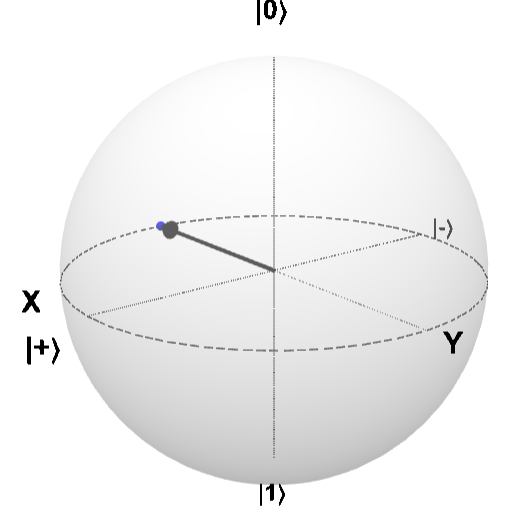
\includegraphics[scale=0.15]{zero-ione}
\caption*{$\kz + e^{i\frac{3\pi}{2}}\ko$}
\end{subfigure}
\end{figure}

\end{frame}

\begin{frame}{Compound Systems}
How do we describe a system composed of two different qubits? As the \textbf{Tensor product} of Hilbert spaces.
\[
	\text{If }\kp, \kf \in \calH \quad\text{ then }\quad \ket{\psi\phi} \in \calH \otimes \calH
\]

$\calH_2 \otimes \calH_2$ is a \textbf{four-dimensional Hilbert space}.
%, and the canonical base is $$\{\kz \otimes \kz, \kz  \otimes \ko, \ko \otimes \kz, \ko  \otimes \ko\}$$ (often written as $\{\ket{00}, \ket{01}, \ket{10}, \ket{11}\}$).

\begin{block}{Dot product in a compound space}
Given $\ket{\psi\psi^\prime}$ and $\ket{\phi\phi^\prime}$, the dot product is defined as
\[
	\braket{\psi\psi^\prime|\phi\phi^\prime} = \braket{\psi|\phi}\braket{\psi^\prime\phi^\prime}
\]
\end{block}
\end{frame}

\subsection{Unitary Transformation}	
\begin{frame}%second postulate
	\frametitle{Second Postulate: Unitary Transformations}
	\begin{block}{II Postulate}
	The evolution of a \textbf{closed} quantum system is described by a \textbf{unitary transformation}. That is, the state $\kp$ of the system at time $t_1$ is related to the state $\ket{\psi^\prime}$ of the system at time $t_2$ by a unitary operator $U$ which depends only on $t_1$ and $t_2$:
	$$ \ket{\psi^\prime} = U\kp$$
	\end{block}
	\begin{itemize}
	\pause\item \textbf{Closed}: without interaction with the environment, i.e. without exchanging with the environment any energy, information, etc..
	\pause\item \textbf{Unitary tranformation} on a Hilbert space $\calH_n$: A $n\times n$ matrix such that its \textit{adjoint} it's also its \textit{inverse}:
	\[UU^H = U^HU = UU{^-1} = I
	\] 
	\end{itemize}
	\end{frame}
	
\begin{frame}%preserve inner product
\frametitle{A useful property}
\begin{block}{Unitary Matrices preserve dot product}
Given $\kp$, $\kf$ with dot product $x$, for a unitary matrix $U$ holds:\begin{gather*}
\braket{\psi|\phi} = x \\
\braket{U\psi | U\phi} =  \braket{\psi| U^H  U |\phi} = \braket{\psi|\phi} = x
\end{gather*}
\end{block}
\pause
\begin{block}{Corollary}
If $\kp$ is a unit vector, $U\kp$ will also be a unit vector.
$$\braket{U\psi | U\psi } = \braket{\psi |\psi} =  1$$
\end{block}
\end{frame}	
	
%\begin{frame}%unitaries example
%\frametitle{Unitary transformations on $\calH_2$}
%\begin{align*}
% I &= \begin{pmatrix}
% 1 & 0\\
% 0 & 1
% \end{pmatrix} &I\kz &= \kz &I\ko &= \ko\\
% X &= \begin{pmatrix}
% 0 & 1 \\
% 1 & 0
% \end{pmatrix} &X\kz &= \ko &X\ko &= \kz\\
% H &= \oost\begin{pmatrix}
% 1 & 1 \\
% 1 & -1
% \end{pmatrix} &H\kz &= \kpl &H\ko &= \km
%\end{align*}
%\pause
%\vspace*{-0.3cm}\begin{figure}
%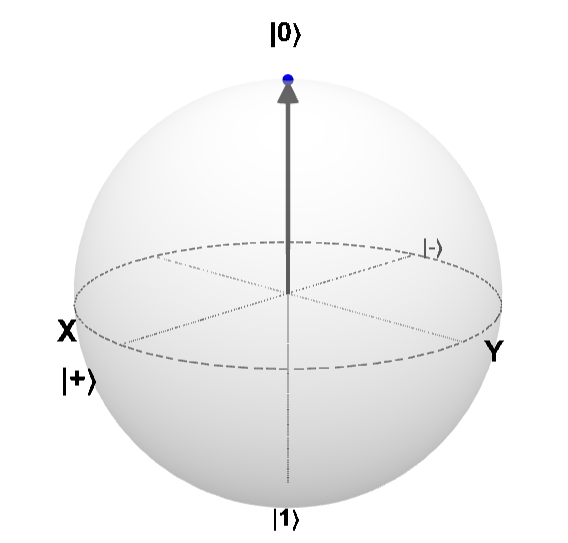
\includegraphics[scale=0.2]{ket0}
%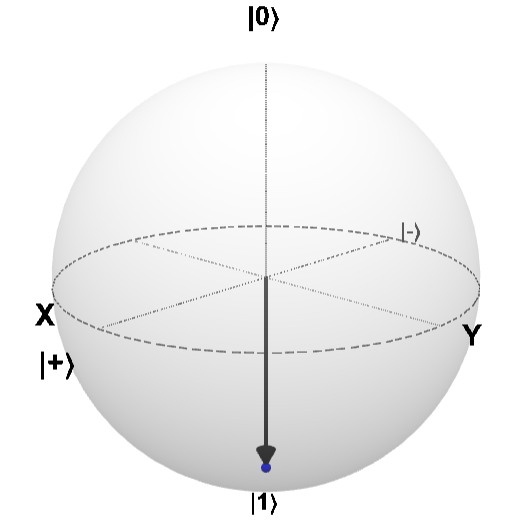
\includegraphics[scale=0.2]{ket1}
%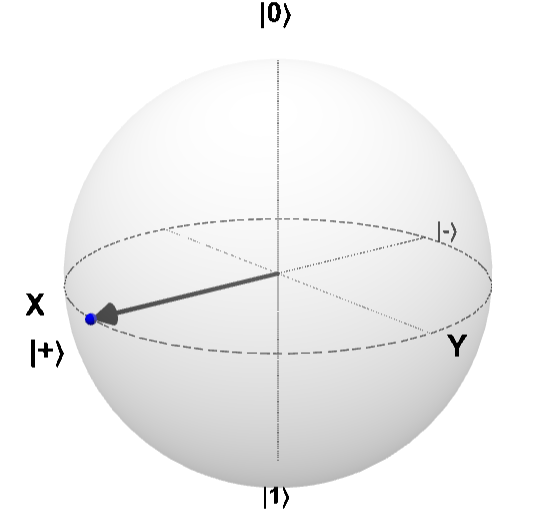
\includegraphics[scale=0.34]{ket+}
%\end{figure}
%\end{frame}

\subsection{Measurements}	
\begin{frame}{Third Postulate: Measurements}
\begin{block}{III Postulate}
	If a state $\kp = \alpha\ket{b_0} + \beta\ket{b_1}$ gets \textbf{measured} in the base $\{b_0, b_1\}$, 
	it will \textbf{collapse} \begin{itemize}
	 \item In state $\ket{b_0}$ with probability $\|\alpha\|^2$
	 \item In state $\ket{b_1}$ with probability $\|\beta\|^2$.
	\end{itemize}
\end{block}


\pause
If $\kz$ gets measured in the computational basis $\{\kz, \ko\}$, it will \textbf{always} result in $\kz$.


\pause\bigskip
If $\kpl = \oost\kz + \oost\ko$ gets measured in the computational basis $\{\kz, \ko\}$, it will result in $\kz$ or $\ko$ with probability $0.5$ each. 


\pause\bigskip
Since $\kz = \oost \kpl + \oost \km$, measuring $\kz$ in the hadamard basis $\{\kpl, \km\}$ will result in $\kpl$ or $\km$ with probability $0.5$ each. 
\end{frame}


%\begin{frame}%third postulate
%	\frametitle{Third Postulate: Measurements}
%
%\begin{block}{III Postulate}
%Quantum measurements are described by a collection $\{M\}_m$ of
%\textbf{measurement operators}, there $m$ are the measurements outcomes.
%If the state of the quantum system is $\kp$, then the \textbf{probability} that result $m$ occurs is 
%\[p(m) = \braket{\psi|M_m^HM_m|\psi} \]
%and the \textbf{state} of the system after the measurement is
%\[ \frac{M_m\kp}{\sqrt{p(m)}}
%\]
%The measurement operators satisfy the \textbf{completeness} equation:
%\[\sum_m M_m^HM_m = I \pause \quad \Big(\textit{i.e. }\forall \kp. \sum_m p(m) = 1\Big)\]	
%\end{block}
%\end{frame}

%\begin{frame}%measurements egs
%\frametitle{Measurements}
%
%Measurement in the computational basis: $\{M_0, M_1\}$
%$$
%M_0 = \begin{pmatrix}
%1 & 0 \\ 0 & 0
%\end{pmatrix}
%\quad\quad
%M_1 = \begin{pmatrix}
%0 & 0 \\ 0 & 1
%\end{pmatrix}
%$$
%
%When measured, the state $\kz$ goes to $0$ with probability 
%$$p(0) \pause =  \Braket{0 | 
%\begin{pmatrix}
%1 & 0 \\ 0 & 0
%\end{pmatrix}^H
%\begin{pmatrix}
%1 & 0 \\ 0 & 0
%\end{pmatrix}
%|0} \pause = 
%\Braket{\begin{pmatrix}
%1 \\ 0
%\end{pmatrix}| 
%\begin{pmatrix}
%1 & 0 \\ 0 & 0
%\end{pmatrix}
%|\begin{pmatrix}
%1 \\ 0
%\end{pmatrix} } \pause = 1
%$$
%\pause
%When measured, the state $\kp = \alpha\kz + \beta\ko$ goes to $0$ with probability 
%$$p(0) = \Braket{\psi | 
%\begin{pmatrix}
%1 & 0 \\ 0 & 0
%\end{pmatrix}
%|\psi} \pause = 
%\begin{pmatrix}
%\overline{\alpha} & \overline{\beta}
%\end{pmatrix} 
%\begin{pmatrix}
%1 & 0 \\ 0 & 0
%\end{pmatrix}
%\begin{pmatrix}
%\alpha \\ \beta
%\end{pmatrix}  \pause = \overline{\alpha}\alpha = \|\alpha\|^2
%$$
%
%\end{frame}

%\begin{frame}%decay
%\frametitle{Superposition Decay}
%
%What happens if we measure the $\kpl$ state in the computational basis ($\{M_0, M_1\}$)?
%\[
% p(0) = \Big\|\oost\Big\|^2 = \frac{1}{\sqrt{2}^2} = 0.5 \quad
% p(1) = \Big\|\oost\Big\|^2 = \frac{1}{\sqrt{2}^2} = 0.5 \quad
%\]
%
%With equal probability, will go in 
%$$\frac{M_0\kpl}{\sqrt{p(0)}} = \sqrt{2}\begin{pmatrix}
%1 & 0 \\ 0 & 0
%\end{pmatrix} \oost \begin{pmatrix} 1 \\ 1 \end{pmatrix} = \begin{pmatrix}
%1 \\ 0
%\end{pmatrix} = \kz 
%$$
%
%$$
%\frac{M_1\kpl}{\sqrt{p(1)}} = \sqrt{2}\begin{pmatrix}
%0 & 0 \\ 0 & 1
%\end{pmatrix} \oost \begin{pmatrix} 1 \\ 1 \end{pmatrix} = \begin{pmatrix}
%0 \\ 1
%\end{pmatrix} = \kz 
%$$
%\begin{alertblock}{}
%The same happens if we measure $\kz$ (or $\ko$) in the Hadamard Basis!
%\end{alertblock}
%\end{frame}

\begin{frame}%takeaway
\frametitle{Takeaway}

To understand the quantum cryptographic protocols, two properties will be useful:
\begin{itemize}
\item The evolution of a quantum system is described by  a \textbf{unitary matrix}, and unitary matrices preserve the inner product. 
\item When the $\kz$ and $\ko$ states are \textbf{measured} in the computational basis, will give with probability $1$ the outcome $\kz$ and $\ko$, respectively. When measured in the Hadamard basis, will give outcome $\kpl$ or $\km$ with probability $\frac{1}{2}$ each. The inverse is true for the $\kpl$ and $\km$ states.
\end{itemize}

\end{frame}

\section{Quantum key distribution}
\begin{frame}{Quantum Key Distribution Protocols}
	Two communicating parties, Alice and Bob, want to establish a shared \textbf{secret} $\mathbf{k} \in \{0, 1\}^N, N \geq 0$ for secure communication. They do not share any prior information, but can make use of:
	\begin{itemize}
	\item A \textbf{classical}, (public) channel, that can be \textcolor{green}{passively monitored} but \textcolor{red}{not tampered} with by an attacker.
	\item A \textbf{quantum} channel, that can be \textcolor{green}{tampered} with by an attacker, but by its nature can not be \textcolor{red}{passively monitored}.
	\end{itemize}   
\begin{figure}
\centering
\includegraphics[scale=0.4]{qkd-alice-bob-eve}
\end{figure}
\end{frame}

%\begin{frame}{Main Idea}
%
%	\begin{block}{QKD in general}
%	\begin{itemize}
%	\item Alice will send to Bob a random sequence of \textbf{non-orthogonal qubits}. Bob can measure these qubits: if he measures in the right basis, he will receive the bit sent by Alice, if not, the outcome will be random. 
%	\item Bob and Alice then communicate on the  to \textbf{reconstruct a shared secret}, keeping the bits correctly read by Bob and discarding the others. 
%	\item The \textbf{presence of an eavesdropper Eve can be detected} with probability arbitrarily near to 1, as it's impossible for Eve to monitor the quantum channel without modifying it.
%
%	\end{itemize}
%\end{block}	 	
%
%\pause Why can't Eve passively monitor the quantum channel?
%
%\end{frame}


\begin{frame}{Information gains implies disturbance}
	
	\begin{block}{Theorem}
	In any attempt to
distinguish between two \textbf{non-orthogonal} quantum states, information gain is only
possible at the expense of \textbf{introducing disturbance} to the signal.

	\end{block}	
	
	Eve, having intercepted a qubit $q \in \{\ket{\psi}, \ket{\phi}\}$  would like to apply a unitary transformation  $U$ such that:
	
	\[
		U(\ket{\psi a}) = \ket{\psi b}
	\]\[
		U(\ket{\phi a}) = \ket{\phi b^\prime}
	\]
	
	\pause
	But, since unitary transformation preserve inner products:
	\[
	\braket{\psi a | \phi a} \pause = 
	\braket{\psi|\phi}\braket{a|a} \pause =
	\braket{\psi|\phi}\braket{b|b^\prime} = 
	\braket{\psi b|\phi b^\prime}
	\]
	\pause
	\vspace*{-0.5cm}
	\[
	\braket{a|a} = \braket{b|b^\prime} \pause = 1
	\]
	\pause
	\vspace*{-0.6cm}
	\begin{center}
	$\ket{b}$ and $\ket{b^\prime}$ must be equal!
	\end{center}
	\end{frame}

\section{BB84 protocol}
\begin{frame}{The BB84 Protocol}%first phase

	\textbf{First Phase: Quantum transmission}
	\begin{enumerate}
		\item Alice creates a random string of bits $\mathbf{d} \in \{0, 1\}^n$, and a random string of bases $\mathbf{b} \in \{\boxplus, \boxtimes\}^n$, where $n > N$.
		\pause\item Alice sends to Bob the sequence of qubits $\ket{\phi_{i}} = \ket{\phi_{b_id_i}}$, where		
	\begin{align*}
		&\ket{\phi_{\comp 0}} = \ket{0}  &\ket{\phi_{\diag 0}} = \ket{+} \\
		&\ket{\phi_{\comp 1}} = \ket{1}  &\ket{\phi_{\diag 1}} = \ket{-}
	\end{align*}				
		\pause\item Bob creates a random string of bases $\mathbf{b}^\prime \in \{\comp, \diag\}^n$, and measures each $\ket{\phi_i}$ in the bases $b_i^\prime$. When he measures $\kz$ or $\kpl$, he stores $0$, when he measures $\ko$ or $\km$, he stores $1$. Doing so he obtains a string of bits $\mathbf{d}^\prime \in \{0, 1\}^n$, that will contain some errors with respect to the original $\mathbf{d}$.
	\end{enumerate}
	
	\textbf{Second Phase: Public discussion}	\\
	\hspace{5pt} Alice and Bob will keep only the correct bits, $\mathbf{k} \subseteq \mathbf{b}$
\end{frame}

\begin{frame}{The BB84 Protocol}%second phase

	\textbf{First Phase: Quantum transmission}\\
	\hspace{5pt} Alice has $\mathbf{d}$ and $\mathbf{b}$, Bob has $\mathbf{d}^\prime$ and $\mathbf{b}^\prime$.
	
	\textbf{Second Phase: Public discussion}
		\begin{enumerate}
		\item Alice sends $\mathbf{b}$ over the public channel, Bob confronts it with $\mathbf{b}^\prime$, and answers to Alice the set $S = \{i \mid b_i = b_i^\prime\}$. Only the corresponding qubits have been correctly measured, and the others are discarded.
		\pause\item Alice chooses a subset oh the remaining bits in $\mathbf{d}$ and discloses their values to Bob. For each $d_i$ in this subset, since it holds $b_i = b_i^\prime$, it should be $d_i = d_i^\prime$. If Bob notices discrepancies $d_i \neq d_i^\prime$, eavesdropping is detected.
		\pause\item The shared secret $\mathbf{k} \in \{0, 1\}^N$ is the string of bits in $\mathbf{d} = \mathbf{b}^\prime$ that have not been disclosed at step 2.
		\end{enumerate}	
\end{frame}

\begin{frame}{BB84 Observations}
\begin{itemize}
\item Alice secret, $\mathbf{d}$, is never completely disclosed. Each bit is sent "encrypted" as $\ket{\phi_{b_i d_i}}$ over the quantum channel. Later, the "key" $b_i$ is revealed, but only \textbf{after that the quantum information $\ket{\phi_{b_i d_i}}$ is destroyed}. 

%\item If Eve intercepts a qubit, she can only measure in a random basis, without knowing if the result corresponds to the original qubit or not. She \textbf{gains only partial information} of Alice's secret, but cannot forward an unaltered qubit to Bob. 

\item If Eve guesses the right base each time, her presence is undetectable, but the probability of this event decreases exponentially with $n$.

%\item If the quantum channels are not perfect, \textbf{some discrepancies $d_i \neq d_i^\prime$ are expected} even without eavesdropping. This means that the probability of Eve going undetected is higher.
\end{itemize}
\end{frame}

\begin{frame}{Eavesdropper's attacks}
	\textbf{What can Eve do?} She can intercept every qubit on the channel, measure it, and send to bob a substitute
	
	
	We will examine two different attacks: 
	\begin{itemize}\pause
		\item \textbf{Intercept-Resend attack}: Alice sends qubit $\ket{\psi_{bd}}$, Eve chooses a basis $\hat{b}$, and measures Alice's qubit, obtaining $\hat{d}$. If $\hat{b} = b$, then $\hat{d} = d$, else $\hat{d}$ will be a random bit. Eve will send to Bob $\ket{\psi_{\hat{b}\hat{d}}}$.
		\pause\item \textbf{Random Substitute attack}: Alice sends qubit $\ket{\psi_{bd}}$, Eve chooses a basis $\hat{b}$ and a bit $\hat{d}$, and measures Alice's qubit. If $\hat{b} = b$, then Eve has discovered $d$. Independently from the measurment, Eve will send to Bob $\ket{\psi_{\hat{b}\hat{d}}}$.
	\end{itemize}
\end{frame}

\begin{frame}[fragile]{PRISM Formalization: Channel}
\begin{scriptsize}
\begin{verbatim}
module ChannelResend
ch_state : [0..4];
ch_bas : [0..1];
ch_bit : [0..1];
[aliceput] (ch_state=0) ->
    (ch_state'=1) & (ch_bas'=al_bas) & (ch_bit'=al_bit);
[evemeasure] (ch_state=1) & (ch_bas=eve_bas) -> (ch_state'=2);
[evemeasure] (ch_state=1) & (ch_bas!=eve_bas) -> 
    0.5 : (ch_state'=2) &(ch_bit'=0) +
    0.5 : (ch_state'=2) &(ch_bit'=1);
[eveget] (ch_state=2) -> (ch_state'=3);
[eveput] (ch_state=3) ->
    (ch_state'=4) & (ch_bas'=eve_bas) & (ch_bit'=eve_bit);
[bobget] (ch_state=4) -> (ch_state'=0);
endmodule
\end{verbatim}
\end{scriptsize}
\end{frame}

\begin{frame}[fragile]{PRISM Formalization: Alice}
\begin{scriptsize}
\begin{verbatim}
const int N;
module Alice
al_state : [0..5];
al_index : [1..N];
al_bas : [0..1];
al_bit : [0..1];
[] (al_state=0) & (eve_state>0) -> 
    0.5 : (al_state'=1) & (al_bas'=0) +
    0.5 : (al_state'=1) & (al_bas'=1);
[] (al_state=1) -> 
    0.5 : (al_state'=2) & (al_bit'=0) +
    0.5 : (al_state'=2) & (al_bit'=1);
[aliceput] (al_state=2) -> (al_state'=3);
[reveal] (al_state=3) -> (al_state'=4);
[loop] (al_state=4) & (al_index<N) -> (al_state'=0) & (al_index'=al_index+1);
[loop] (al_state=4) & (al_index=N) -> (al_state'=5);
[stop] (al_state=4) -> (al_state'=4);
[stop] (al_state=5) -> (al_state'=5);
endmodule
\end{verbatim}
\end{scriptsize}
\end{frame}

\begin{frame}[fragile]{PRISM Formalization: Bob}
\begin{scriptsize}
\begin{verbatim}
const int CHECKBIT;
module Bob
bob_state : [0..7];
bob_bas : [0..1];
bob_bit : [0..1];
[] (bob_state=0) & (eve_state>0) -> 
    0.5 : (bob_state'=2) & (bob_bas'=0) +
    0.5 : (bob_state'=2) & (bob_bas'=1);
[bobget] (bob_state=2) & (bob_bas=ch_bas) -> (bob_state'=3) & (bob_bit'=ch_bit);
[bobget] (bob_state=2) & (bob_bas!=ch_bas) -> 
    0.5 : (bob_bit'=ch_bit) & (bob_state'=3) +
    0.5 : (bob_bit'=1-ch_bit) & (bob_state'=3);
[reveal] (bob_state=3) & (bob_bas!=al_bas) -> (bob_state'=4);
[reveal] (bob_state=3) & (bob_bas=al_bas)  -> (bob_state'=5);
[] (bob_state=5) & (bob_bit!=al_bit) -> (bob_state'=7);
[] (bob_state=5) & (bob_bit=al_bit) -> (bob_state'=4);
[loop] (bob_state=4) & (al_index<N) -> (bob_state'=0);
[loop] (bob_state=4) & (al_index=N) -> (bob_state'=6);
[stop] (bob_state=6) -> (bob_state'=6); // no eavesdropping detected
[stop] (bob_state=7) -> (bob_state'=7); // eavesdropping detected
endmodule
\end{verbatim}
\end{scriptsize}
\end{frame}


%\begin{frame}[fragile]{PRISM Formalization: Bob}
%\begin{scriptsize}
%\begin{verbatim}
%const int CHECKBIT;
%module Bob
%bob_state : [0..7];
%bob_bas : [0..1];
%bob_bit : [0..1];
%[] (bob_state=0) & (eve_state>0) -> 
%    0.5 : (bob_state'=2) & (bob_bas'=0) +
%    0.5 : (bob_state'=2) & (bob_bas'=1);
%[bobget] (bob_state=2) & (bob_bas=ch_bas) -> (bob_state'=3) & (bob_bit'=ch_bit);
%[bobget] (bob_state=2) & (bob_bas!=ch_bas) -> 
%    0.5 : (bob_bit'=ch_bit) & (bob_state'=3) +
%    0.5 : (bob_bit'=1-ch_bit) & (bob_state'=3);
%[reveal] (bob_state=3) & (bob_bas!=al_bas) -> (bob_state'=4);
%[reveal] (bob_state=3) & (bob_bas=al_bas)  -> 
%    CHECKBIT: (bob_state'=5) + 
%    1-CHECKBIT: (bob_state' = 4);
%[] (bob_state=5) & (bob_bit!=al_bit) -> (bob_state'=7);
%[] (bob_state=5) & (bob_bit=al_bit) -> (bob_state'=4);
%[loop] (bob_state=4) & (al_index<N) -> (bob_state'=0);
%[loop] (bob_state=4) & (al_index=N) -> (bob_state'=6);
%[stop] (bob_state=6) -> (bob_state'=6); // no eavesdropping detected
%[stop] (bob_state=7) -> (bob_state'=7); // eavesdropping detected
%endmodule
%\end{verbatim}
%\end{scriptsize}
%\end{frame}

\begin{frame}[fragile]{PRISM Formalization: Intercept/Resend}
\begin{footnotesize}
\begin{verbatim}
module EveResend
eve_state : [0..4];
eve_bas : [0..1];
eve_bit : [0..1];
[] (eve_state=0) -> 
    0.5 : (eve_state'=1) & (eve_bas'=0) + 
    0.5 : (eve_state'=1) & (eve_bas'=1);
[evemeasure] (eve_state=1) -> (eve_state'=2);
[eveget] (eve_state=2)  -> (eve_state'=3) & (eve_bit'=ch_bit) ;
[eveput] (eve_state=3) -> (eve_state'=0);
endmodule
\end{verbatim}
\end{footnotesize}
\end{frame}

\begin{frame}[fragile]{PRISM Formalization: Random Substitution}
\begin{footnotesize}
\begin{verbatim}
module EveRandom
eve_state : [0..4];
eve_bas : [0..1];
eve_bit : [0..1];
[] (eve_state=0) -> 
    0.5 : (eve_state'=1) & (eve_bas'=0) + 
    0.5 : (eve_state'=1) & (eve_bas'=1);
[evemeasure] (eve_state=1) -> (eve_state'=2);
[eveget] (eve_state=2)  -> (eve_state'=3) & (eve_bit'=ch_bit) ;
[] (eve_state=3) ->
    0.50: (eve_state'=4) & (eve_bit'=0) +
    0.50: (eve_state'=4) & (eve_bit'=1) ;
[eveput] (eve_state=4) -> (eve_state'=0);
endmodule
\end{verbatim}
\end{footnotesize}
\end{frame}

\begin{frame}{Eve will be detected}
\includegraphics[scale=0.46]{prism/BB84_rand_vs_resend}
\pause
\includegraphics[scale=0.46]{prism/EveDet_bb84_resend}
\end{frame}


\section{B92 Protocol}

\begin{frame}{The B92 Protocol}%first phase

	\textbf{First Phase: Quantum transmission}
	\begin{enumerate}
		\item Alice creates a random string of bits $\mathbf{b} \in \{\comp, \diag\}^n$, where $n > N$.
		\item Alice sends to Bob the sequence of qubits $\ket{\phi_{i}} = \ket{\phi_{b_i}}$, where		
	\begin{align*}
		&\ket{\phi_\comp} = \ket{0}  &\ket{\phi_\diag} = \ket{+}
	\end{align*}				
		\pause\item Bob creates a random string of bases $\mathbf{b}^\prime \in \{\comp, \diag\}^n$, and measures each $\ket{\phi_i}$ in the bases $b_i^\prime$. Doing so he construct a sequence of bits $\mathbf{t} \in \{0, 1\}^N$, such that
	\[ t_i = 
	\begin{cases}
	0 \text{ if $\ket{\phi_i}$, measured with $b_i^\prime$, yields $\ket{0}$ or $\ket{+}$} \\
	1 \text{ if $\ket{\phi_i}$, measured with $b_i^\prime$, yields $\ket{1}$ or $\ket{-}$}
	\end{cases}
	\]
	\end{enumerate}
	
	\textbf{Second Phase: Public discussion}	\\
	\hspace{5pt} Alice and Bob will keep only the correct bits, $\mathbf{k} \subseteq \mathbf{b}$
\end{frame}


	\begin{frame}{The B92 Protocol}%second phase

	\textbf{First Phase: Quantum transmission}\\
	\hspace{5pt} Alice has $\mathbf{b}$, Bob has $\mathbf{b}^\prime$ and $\mathbf{t}$
	
	\textbf{Second Phase: Public discussion}
		\begin{enumerate}
		\item When $t_i = 1$, it means that Bob has used the wrong basis, and so he knows the original bit $b_i$, that is $1 - b_i^\prime$. Bob sends $\mathbf{t}$ over the public channel, and both parties keep only the bits for which $t_i = 1$.
		\pause\item Alice chooses a subset oh the remaining bits in $\mathbf{b}$ and discloses their values to Bob. For each $b_i$ in this subset, it should be $b_i = 1-b_i^\prime$. If Bob notices discrepancies $b_i = b_i^\prime$, eavesdropping is detected.
		\item The shared secret $\mathbf{k} \in \{0, 1\}^N$ is the string of bits in $\mathbf{b} = \mathbf{1-b}^\prime$ that have not been disclosed at step 2.
		\end{enumerate}	
\end{frame}

\begin{frame}{B92 Observation}

\begin{itemize}
\item Alice secret, $\vec{d}$, is never completely disclosed. Each bit is sent codified in a quantum state ($\ket{0}$ or $\ket{+}$), but these two state are not distinguishable without altering them.

\item If Bob guesses the right base, he gains no information. If he uses the wrong base, he could measure a state in $\{\ket{0}, \ket{+}\}$, which gives him no information, or a state in $\{\ket{1}, \ket{-}\}$, which is surely an error. He so can deduce the basis that Alice was using.

\item With respect to BB84, B92 discards more bits, as the probability of Bob gaining information is $\frac{1}{4}$.
\end{itemize}

\end{frame}

\begin{frame}[fragile]{PRISM Formalization: Alice}
\begin{scriptsize}
\begin{verbatim}
module Alice
al_state : [0..5];
al_index : [1..N];
al_bas : [0..1];
al_bit : [0..1];
[] (al_state=0) & (eve_state>0) -> 
	0.5 : (al_state'=1) & (al_bit'=0) & (al_bas'=0)+
	0.5 : (al_state'=1) & (al_bit'=0) & (al_bas'=1);
[aliceput] (al_state=1) -> (al_state'=2);
[reveal] (al_state=2) -> (al_state'=3);
[loop] (al_state=3) & (al_index<N) -> (al_state'=0) & (al_index'=al_index+1);
[loop] (al_state=3) & (al_index=N) -> (al_state'=4);
[stop] (al_state=3) -> (al_state'=3);
[stop] (al_state=4) -> (al_state'=4);
endmodule
\end{verbatim}
\end{scriptsize}
\end{frame}


\begin{frame}[fragile]{PRISM Formalization: Bob}
\begin{scriptsize}
\begin{verbatim}
module Bob
bob_state : [0..7];
bob_bas : [0..1];
bob_bit : [0..1];
[] (bob_state=0) & (eve_state>0) -> 
    0.5 : (bob_state'=2) & (bob_bas'=0) +
    0.5 : (bob_state'=2) & (bob_bas'=1);
[bobget] (bob_state=2) & (bob_bas=ch_bas) -> (bob_state'=3) & (bob_bit'=ch_bit);
[bobget] (bob_state=2) & (bob_bas!=ch_bas) -> 
    0.5 : (bob_bit'=ch_bit) & (bob_state'=3) +
    0.5 : (bob_bit'=1-ch_bit) & (bob_state'=3);
[reveal] (bob_state=3) & (bob_bit = 0) -> (bob_state'=4);
[reveal] (bob_state=3) & (bob_bit = 1)  ->  (bob_state' = 5);
[] (bob_state=5) & (bob_bas != 1 - al_bas) -> (bob_state'=7);
[] (bob_state=5) & (bob_bas = 1 - al_bas) -> (bob_state'=4);
[loop] (bob_state=4) & (al_index<N) -> (bob_state'=0);
[loop] (bob_state=4) & (al_index=N) -> (bob_state'=6);
[stop] (bob_state=6) -> (bob_state'=6); // no eavesdropping detected
[stop] (bob_state=7) -> (bob_state'=7); // eavesdropping detected
endmodule
\end{verbatim}
\end{scriptsize}
\end{frame}

%\begin{frame}[fragile]{PRISM Formalization: Bob}
%\begin{scriptsize}
%\begin{verbatim}
%module Bob
%bob_state : [0..7];
%bob_bas : [0..1];
%bob_bit : [0..1];
%[] (bob_state=0) & (eve_state>0) -> 
%    0.5 : (bob_state'=2) & (bob_bas'=0) +
%    0.5 : (bob_state'=2) & (bob_bas'=1);
%[bobget] (bob_state=2) & (bob_bas=ch_bas) -> (bob_state'=3) & (bob_bit'=ch_bit);
%[bobget] (bob_state=2) & (bob_bas!=ch_bas) -> 
%    0.5 : (bob_bit'=ch_bit) & (bob_state'=3) +
%    0.5 : (bob_bit'=1-ch_bit) & (bob_state'=3);
%[reveal] (bob_state=3) & (bob_bit = 0) -> (bob_state'=4);
%[reveal] (bob_state=3) & (bob_bit = 1)  -> 
%    CHECKBIT: (bob_state' = 5) + 
%    1-CHECKBIT: (bob_state' = 4);
%[] (bob_state=5) & (bob_bas != 1 - al_bas) -> (bob_state'=7);
%[] (bob_state=5) & (bob_bas = 1 - al_bas) -> (bob_state'=4);
%[loop] (bob_state=4) & (al_index<N) -> (bob_state'=0);
%[loop] (bob_state=4) & (al_index=N) -> (bob_state'=6);
%[stop] (bob_state=6) -> (bob_state'=6); // no eavesdropping detected
%[stop] (bob_state=7) -> (bob_state'=7); // eavesdropping detected
%endmodule
%\end{verbatim}
%\end{scriptsize}
%\end{frame}



	
\section{Comparison}
\begin{frame}{BB84 and B92}
\includegraphics[scale=0.46]{prism/BB84_rand_vs_resend}
\includegraphics[scale=0.46]{prism/b92_rand_vs_resend}
\end{frame}
	
\begin{frame}[fragile]{A smarter MIM attack}
\begin{footnotesize}
\begin{verbatim}
module EveClever
eve_state : [0..4];
eve_bas : [0..1];
eve_bit : [0..1];
[] (eve_state=0) -> 
    0.5 : (eve_state'=1) & (eve_bas'=0) + 
    0.5 : (eve_state'=1) & (eve_bas'=1);
[evemeasure] (eve_state=1) -> (eve_state'=2);
[eveget] (eve_state=2)  -> (eve_state'=3) & (eve_bit'=ch_bit) ;
[] (eve_state=3) & (eve_bit = 1) -> 
    (eve_bas'=1-eve_bas) & (eve_bit'=0) & (eve_state' = 4);
[] (eve_state=3) & (eve_bit = 0) -> 
    (eve_bas'=eve_bas) & (eve_bit'=0) & (eve_state' = 4);
[eveput] (eve_state=4) -> (eve_state'=0);
endmodule
\end{verbatim}
\end{footnotesize}
\end{frame}

\begin{frame}{BB84 and B92}
\includegraphics[scale=0.46]{prism/BB84_rand_vs_resend}
\includegraphics[scale=0.46]{prism/b92_rand_vs_resend_adj}
\end{frame}

\begin{frame}{Other interesting metrics: bits obtained by Eve}
\includegraphics[width=\textwidth]{eve_bits}
\end{frame}

\begin{frame}{Other interesting metrics: Eve with different power}
\centering
\includegraphics[scale=0.28]{eve_powers}
\end{frame}

\begin{frame}{Bibliography}
\nocite{*}
\bibliographystyle{abbrv} % We choose the "plain" reference style
{\footnotesize \bibliography{bibliografia}} 
\end{frame}
\end{document}
